\chapter*{Bilagor}
\addcontentsline{toc}{chapter}{Bilagor}
\appendix

\chapter{Himmelssfären och astronomiska koordinatsystem}
\label{app:coord}

\section{En position på jorden}

Jordekvatorn definieras som storcirkeln som ligger halvägs mellan
nord- och sydpolen. Meridianen definierades 1884 som den halvcirkel
som går genom polerna och ``Old Royal Observatory'' i Greenwich,
Storbrittannien. 

En position på jordens yta är unikt bestämd av tre storheter:
longituden $\lambda$, latituden $\phi$, samt höjden över havsytan,
$h$. Longituden mäts västerut från meridianen till den punkt där
longitudcirkels korsar ekvatorn. Latituden är positiv på norra
halvklotet och negativ på det södra, och definieras som vinkeln längs
longitudcirkeln från ekvatorn till den aktuella positionen.

Onsala Rymdobservatorium ligger några meter över havsytan och har
följande longitud och latitud, respektive:

\begin{center}
${{\boxed{\lambda=12^{\circ}01'00'' \text{E}
\hspace{1cm}\phi=57^{\circ}25'00''\text{N.} }}}$
\end{center}  

\begin{figure}[ht]
\begin{center}
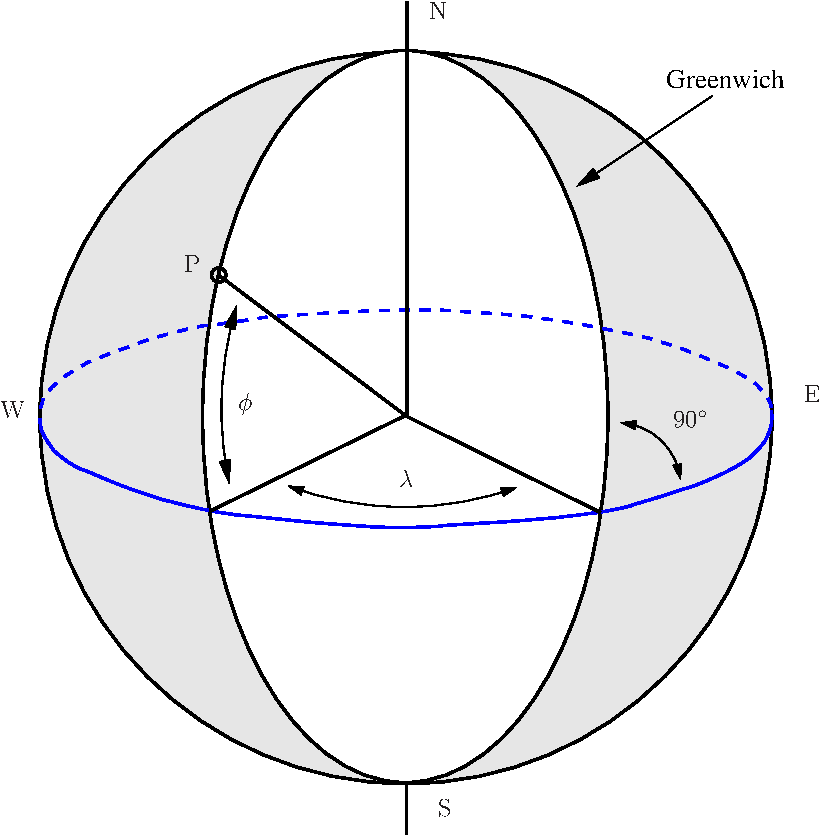
\includegraphics[width=8cm]{../figures/longlat.pdf}
\end{center}
\caption{Illustration av longitud ($\lambda$) och latitud ($\phi$) på
  jorden. Storcirklar som går genom polerna är
  longitudcirklar. Cirklar som är parallella med ekvatorn är
  latitudcirklar. }
\label{figearth}
\end{figure}


\section{Himmelsfären}

\subsection{Ekvatoriella koordinater}

\begin{figure}[ht]
\begin{center}
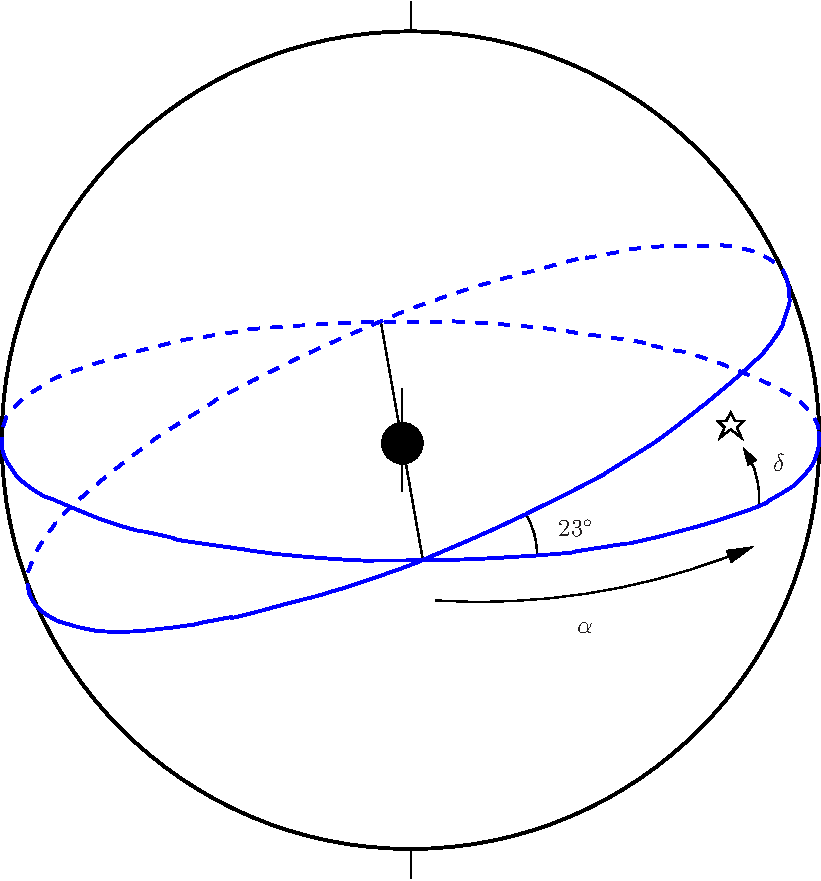
\includegraphics[width=8cm]{../figures/celestial.pdf}
\end{center}
\caption{Det ekvatoriella koordinatsystemet, med RA $\alpha$ och
  deklination $\delta$. Jorden ligger i centrum. Ekliptikans plan
  lutar 23.5$^\circ$ jämfört med jordens ekvator.}
\label{figcelest}
\end{figure}

Himmelsfären är en inbillad sfär som är koncentrisk med Jorden. På
denna sfär är de astronomiska objekten placerade (se
Fig.~\ref{figcelest}). Himmelsekvatorn är de naturliga förlängningen
av jordekvatorn. Eftersom jordens rotationsaxel lutar 23.5 grader
jämfört med solsystemsplanet sammanträffar inte ekliptikan (solens
banplan) med himmelsekvatorn. Punkten där Solen korsar himmelsekvatorn
på väg norrut kallas Vårdagjämningnen och inträffar runt den 21
mars. Då ligger solen i jordens ekvatorialplan och dag och natt är
lika långa. På väg söderut passerar sedan Solen himmelsekvatorn igen
den 21 september (höstdagjämningen). Sommar- och vintersolstånden
inträffar då solen är längst bort från himmelsekvatorn och inträffar
21 juni respektive 21 december.

\medskip
{{$\rightarrow$ Markera norra och södra himmelspolen,
    himmelsekvatorn , ekliptikan, solstånden samt vår- och
    höstdagjämningarna i Fig.~\ref{figcelest}.}}
\medskip

Positioner på himmelssfären definieras av vinklar längs
storcirklar. Himmelslongituden (rektascension, RA) $\alpha$ för ett
astronomiskt objekt definieras i analogi med longitud på jorden. Den
mäts österut från vårdagjämningen längs himmelsekvatorn. RA uttrycks i
timmar, minuter och sekunder där 24 timmar motsvarar hela varvet,
360$^\circ$.

I analogi med latitud definieras himmelslatitud (deklinationen) som
vinkelavståndet till ett objekt från himmelsekvatorn. Tillsammans
bestämmer RA och deklinationen fullständigt en posiition på
himmelssfären.

Tänk dig nu att vi befinner oss på en plats $P$ på jorden vid
latituden $\phi$, och att vi vill observera himlen. Ett astronomiskt
objekt med deklinationen $\delta$ når då sin maximala höjd över
horisonten $h_{\rm max}$, och minimala höjd $h_{\rm min}$ enligt

\begin{equation}
\begin{array}{l}
h_{\rm max} = 90^\circ -|\phi-\delta| \\
h_{\rm min} = -90^\circ +|\phi+\delta|. 
\end{array}
\end{equation}

{{$\rightarrow$ I Onsala stannar alltid astronomiska
    objekt med $\delta > 33^\circ$ 
alltid över horisonten (de är circumpolära); }}

{{$\rightarrow$ de med $\delta < -33^\circ$ kommer aldrig
    över horisonten.}}


\subsection{Den lokala stjärntiden}

\begin{figure}[ht]
\begin{center}
 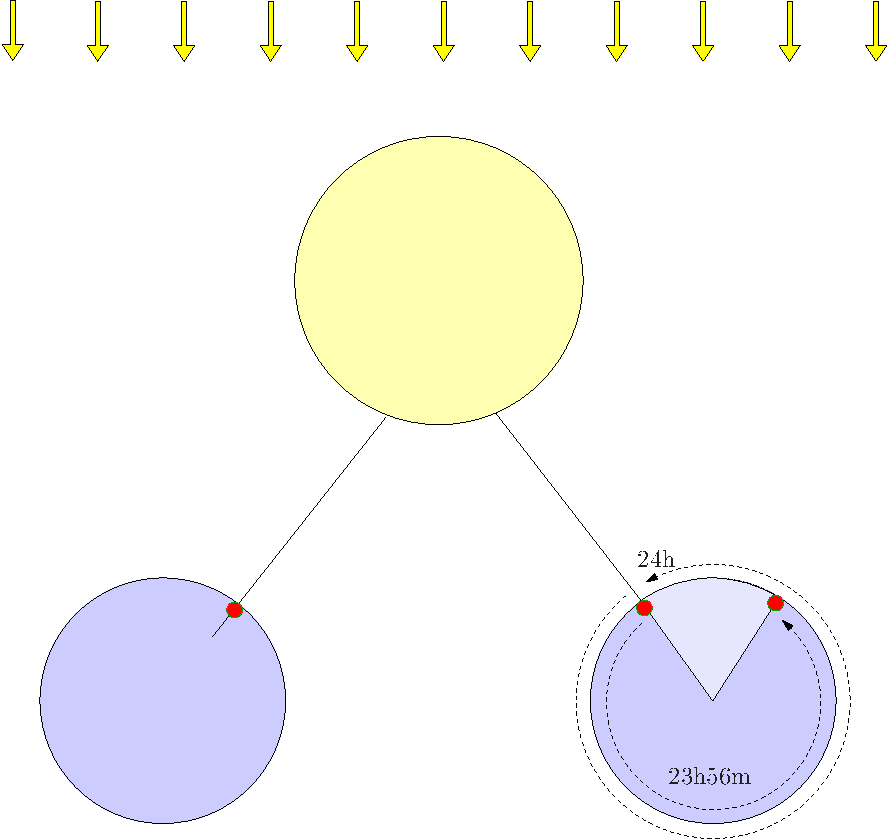
\includegraphics[width=8cm]{../figures/lst.pdf}
\end{center}
\caption{Den lokala stjärntiden (LST) är definierad relativt
  stjärnorna, medan soltiden definieras relativt solen. 24~timmar
  LST-tid motsvarar bara 23~timmar 56~minuter 05~sekunder soltid.}
\label{figlst}
\end{figure}

Anledningen till att man mäter RA österut är att det gör himmelsfären
till en urtavla. Visaren är den \textbf{lokala meridianen} (nord-syd
linjen som går genom observatörens zenith).


Vid vårdagjämningen är den lokala stjärntiden (LST) 0 timmar. Detta
inträffar klockan tolv (soltid).

När tiden går kommer astronomiska objekt på den lokala meridianen ha
en större RA. Vid varje tillfälle och vid varje plats på jorden är
alltid LST lika med RA för de astronomiska objekten på den lokala meridianen.

``Himmelsklockan'' går fortare än solklockan varje dag. Detta kommer
sig av att jorden roterar både runt sin egen axel och runt solen,
vilket illustreras i figur~\ref{figlst}. Efter 24 timmar soltid har en
plats på jorden samma soltid igen (ett dygn). Men 24 timmar stjärntid
går ungefär fyra sol-minuter fortare, eftersom vi inte behöver vrida
oss lika långt för att komma till samma position relativt
stjärnorna. 24 timmar LST motsvarar därför 23 timmar 56 minuter och 5
sekunder soltid. Varje dag inträffar en LST tid fyra minuter (soltid)
tidigare än dagen innan.

Vid vårdagjämningen är alltså LST 0h vid soltiden 12h. Nästa dag vid
12h soltid är LST 0h 3min 56s. För varje månad inträffar en LST tid 2
timmar tidigare.

\subsection{Hur kan jag veta om min källa är synlig?}
\label{app:visiblecoords}

Anta att vi vill observera i en viss riktning i det galaktiska planet
(en viss longitud $l$ och latitud $b=0$), vid en viss tidpunkt.

Först måste vi konvertera Våra galaktiska koordinater till
ekvatoriella koordinater (RA \& DEC). För att förenkla har vi räknat
ut RA \& DEC för ett antal galaktiska longituder i planet. Dessa finns i tabell \ref{tab:radec}. 

Som vi redan sett kan man inte observera källor som alltid ligger under
horisonten i Onsala (de med $\delta < -33^\circ$).

Det bästa sättet att lära sig hur det fungerar är att studerar några exempel!

\bigskip {\bf Example~1.} Idag är julafton och jag har tillgång till
ett litet optiskt teleskop. Jag skulle vilja observera den vackra
``virvelgalaxen'' M51. Är det möjligt? 

\smallskip M51 har koordinaterna $\alpha\simeq13$~h~30m,
$\delta\simeq+47^\circ$. Det betyder att M51 kommer att vara som högst
över horisonten vid LST=13~h~30.

LST= 0~h vid = 12~h den 21 mars.

LST= 0~h vid $12-(2\times 9) = -6$~h (eller $24-6=18$~h) runt 21 dec
eftersom det är nio månader efter den 21 Mars, och LST går 2 timmar
fortare varje månad.

LST=13~h~30 vid 18+13~h~30= 7~h~30.

M51 kommer att vara som högst på himlen på morgonen klockan 7h30 och
kommer att stiga under den andra delen av natten,

\begin{table}
\label{tabcoord}
\begin{center}
\begin{tabular}{rrr}
\hline
\medskip
$l$ & $\alpha(J2000)$ &$\delta(J2000)$\\
$^\circ$ &h m &$^\circ\,\,\,\,\,$$'$\\
\hline
0 & 17h45 & --28:56 \\
20 & 18h27 & --11:29 \\
40 & 19h04 & 06:17 \\
60 & 19h43 & 23:53 \\
{\bf\green 80}  & 20h35 & 40:39\\
{\bf\green 100} & 22h00 & 55:02\\
{\bf\green 120} & 00h25 & 62:43 \\
{\bf\green 140} & 03h07 & 58:17 \\
{\bf\green 160} & 04h46 & 45:14\\
180 & 05h45 & 28:56\\
200 & 06h27 & 11:29\\
220 & 07h04 & --06:17\\
240 & 07h43 & --23:53\\
\red 260 & 08h35 & --40:39\\
\red 280 & 10h00 & --55:02\\
\red 300 & 12h25 & --62:43\\
\red 320 & 15h07 & --58:17\\
\red 340 & 16h46 & --45:14\\
\hline
\end{tabular}
\caption{Konversion mellan galaktiska koordinater till ekvatoriella
  koordinater för olika $l$ med $b=0$. Longituderna i grön fetstil är
  cirkumpolära i Onsala, och de i rött kommer aldrig över horisonten.
\label{tab:radec}
}
\end{center}
\end{table}
